%          spconf.sty  - ICASSP/ICIP LaTeX style file, and
%          IEEEbib.bst - IEEE bibliography style file.
% --------------------------------------------------------------------------
\documentclass{article}
\usepackage{spconf,amsmath,graphicx,tabularx}
\usepackage{booktabs}

\usepackage{hyperref}
\usepackage{amssymb}


% Title.
% ------
\title{Navigating Challenges and Opportunities: AI in Medical Imaging}
\name{SN: 24076677}
\address{}
%
\begin{document}
%
\maketitle
\section{Scope and Focus Areas}
This blog will explore the transformative potential of artificial intelligence (AI) in healthcare, with a concentrated focus on medical imaging—a domain where AI promises to revolutionize diagnostics, treatment planning, and patient outcomes. However, the blog will critically examine the barriers hindering widespread adoption, particularly data scarcity and privacy concerns. Specific sectors of focus include:

\subsection{Data Scarcity in Medical Imaging}
Medical imaging AI models require vast, diverse datasets to achieve high accuracy. However, acquiring such data is fraught with difficulties:
\begin{itemize}
    \item \textbf{Annotated Data Limitations}: Unlike general-purpose images (e.g., photographs), medical scans demand expert annotations (e.g., radiologists labeling tumors), which are time-consuming and costly. For rare diseases, such as pediatric cancers or genetic disorders, datasets may consist of only a few hundred cases—insufficient for robust model training.
    \item \textbf{Bias and Representativeness}: Many publicly available datasets skew toward populations in high-income countries, leading to models that underperform for underrepresented groups. For example, a 2023 study revealed that melanoma detection algorithms trained predominantly on lighter skin tones showed 30\% lower accuracy for darker-skinned patients.
\end{itemize}

\subsection{Privacy Concerns and Regulatory Hurdles}
Medical imaging data is inherently sensitive, often containing personally identifiable information (PII). Strict regulations like the EU’s General Data Protection Regulation (GDPR) and the U.S. Health Insurance Portability and Accountability Act (HIPAA) restrict data sharing across institutions, stifling collaboration. Even anonymization techniques, such as removing patient metadata, may fail to prevent re-identification—a risk highlighted by the 2024 breach of a de-identified MRI database in Germany.

\section{Machine Learning Technologies to be Explored}
The blog will analyze cutting-edge ML methodologies designed to mitigate data and privacy challenges:
\subsection*{1. Federated Learning: Collaboration Without Data Sharing}
Federated learning (FL) enables hospitals to collaboratively train AI models without exchanging raw data. Instead, models are trained locally on institutional servers, and only model updates (not patient data) are shared. For example, \textbf{NVIDIA Clara’s FL platform} has been adopted by 20+ U.S. hospitals to improve liver tumor segmentation accuracy by 15\% while maintaining compliance with HIPAA. However, FL faces challenges, including computational overhead and ensuring consistent data quality across sites.

\subsection*{2. Synthetic Data: Bridging the Gap with AI-Generated Scans}
Generative adversarial networks (GANs) and diffusion models are being used to create synthetic medical images that mimic real patient data. Projects like \textbf{MIT’s SynthMed} have generated synthetic brain MRIs with realistic tumors, enabling researchers to augment small datasets. While promising, synthetic data risks perpetuating biases if the original training data is unrepresentative.

\subsection*{3. Transfer Learning and Self-Supervised Learning}
Transfer learning allows models pretrained on non-medical datasets (e.g., ImageNet) to be fine-tuned for medical tasks with limited data. For instance, Google’s \textbf{CheXpert} model, pretrained on chest X-rays, achieved state-of-the-art pneumonia detection with 50\% fewer labeled examples. Similarly, self-supervised learning techniques like contrastive learning (e.g., \textbf{SimCLR}) leverage unlabeled data to extract meaningful features, reducing reliance on annotations.

\subsection*{4. Privacy-Preserving Techniques}
Differential privacy (DP) adds mathematical “noise” to datasets or model outputs to prevent re-identification. Apple’s \textbf{DP-SGD} framework, for example, has been adapted to train mammography classifiers with provable privacy guarantees. Meanwhile, \textbf{homomorphic encryption} allows computations on encrypted data, though its computational demands remain a barrier for real-time imaging applications.

\begin{figure}[htb]
    \centering
    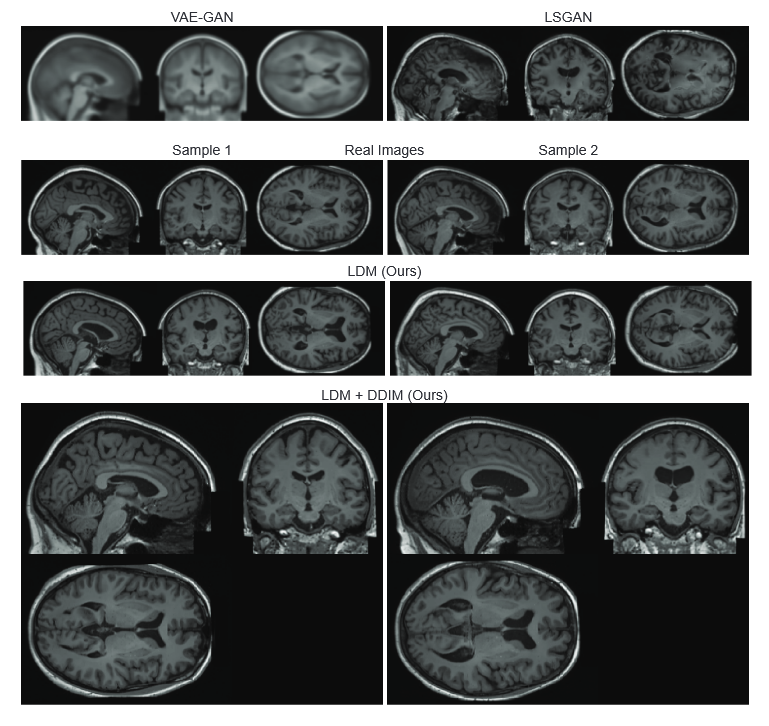
\includegraphics[width=0.48\textwidth]{images/generation.png}
    \caption{Synthetic data generation using GANs.}
    \label{fig:generation}
\end{figure}

\section{Wider Issues to be Discussed}

Beyond technical challenges, the blog will address ethical, regulatory, and societal implications:

\subsection*{1. Ethical Dilemmas in AI-Driven Diagnostics}
\begin{itemize}
    \item \textbf{Bias and Fairness}: AI models trained on biased data risk exacerbating healthcare disparities. For example, a 2024 audit of commercial AI radiology tools found that lung nodule detection accuracy dropped by 22\% for Asian patients compared to Caucasian cohorts. Mitigating this requires inclusive dataset curation and algorithmic fairness frameworks like IBM’s \textbf{AI Fairness 360}.
    \item \textbf{Accountability}: When an AI system misdiagnoses a condition, liability becomes murky. Should responsibility lie with the clinician using the tool, the developer, or the hospital? Legal precedents are still evolving.
\end{itemize}

\subsection*{2. Regulatory Frameworks and Global Standards}
Regulators are racing to keep pace with AI innovation. The FDA’s \textbf{Software as a Medical Device (SaMD)} guidelines now mandate rigorous validation for AI tools, including real-world performance monitoring. In the EU, the proposed \textbf{AI Act} classifies medical imaging AI as “high-risk,” requiring transparency reports and human oversight. However, low-resource regions often lack such frameworks, leading to unregulated deployment of unreliable tools.

\subsection*{3. Patient Trust and Transparency}
Public skepticism remains a barrier. A 2025 survey by the Pew Research Center found that 62\% of patients distrust AI for critical diagnoses, citing “black box” decision-making. Explainable AI (XAI) tools like \textbf{LIME} and \textbf{SHAP} aim to demystify predictions by highlighting regions of interest in scans (e.g., showing which pixels influenced a tumor classification). Clinician education is equally vital; radiologists must understand AI’s limitations to avoid overreliance.

\subsection*{4. Economic and Workforce Impact}
While AI could alleviate radiologist shortages in underserved areas (e.g., sub-Saharan Africa has <1 radiologist per 100,000 people), fears of job displacement persist. However, studies suggest AI will augment rather than replace radiologists, automating repetitive tasks (e.g., measuring tumor volumes) and freeing experts for complex cases. 

Proposed Structure for Full Blog:
\begin{enumerate}
    \item Introduction to AI in Medical Imaging
    \item Technical Challenges: Data Scarcity \& Privacy
    \item Innovative ML Solutions
    \item Ethical, Legal, and Social Implications
    \item Global Case Studies
    \item The Path Forward
\end{enumerate}

\end{document}
